\documentclass{report}
\usepackage[tmargin=2cm, rmargin=1in, lmargin=1in,margin=0.85in,bmargin=2cm,footskip=.2in]{geometry}
\usepackage{amsmath,amsfonts,amsthm,amssymb,mathtools}
\usepackage{enumitem}
\usepackage[]{mdframed}
\usepackage{tikz}
\usepackage[style=ieee]{biblatex}


\graphicspath{ {figures/} }

\addbibresource{FinalEssay.bib}

\title{\Huge{Math 181}\\Kepler's Six Cornered Snowflake}
\author{\huge{Elijah Hantman}}
\date{}

\begin{document}
\maketitle
\newpage

In 1611 Johannes Kepler wrote a small latin essay for his friend and benefactor Counselor Wackher von Wackenfels titled 
“A New Year’s Gift, or On The Six Cornered Snowflake”\cite[p.xi]{kepflake}. In it, Kepler attempts to grapple with the 
question of why snowflakes are hexagonal a deceptively difficult question that will birth entirely new fields of 
scientific study. It is a work which is in the same tradition as The Sand Reckoner by Archimedes, 
a piece of mathematical writing which serves the purpose of demonstrating mathematical thought to laypeople as well as
being a glimpse into the culture of mathematics and the minds of their authors.

Kepler begins by discussing what he could give his friend for the New Year. He eventually arrives on the question of Why Snowflakes are Hexagonal \cite[p.7]{kepflake}
as his gift. To begin, Kepler asks two questions, Why do Bees make Hexagonal cells, and why do Pomegranate Seeds form Hexagonal three Dimensional patterns?

Pomegranate seeds form dodecahedrons which have embedded hexagons. A more theological and descriptive approach would be about the
beauty of these solids, and how there are geometric ways to extract the golden ratio from these shapes. The golden ratio being an
extremely interesting and profound number involved in both geometry as well as algebra.

Instead Kepler begins by connecting the pomegranate problem to an experiment you can do involving squishing soft balls. Kepler notes
that not all pomegranate seeds are what are known as rhombic dodecahedrons. Rather, only the seeds in the center of large full 
pomegranates are dodecahedrons, outer seeds are instead spheres. Experimentally when you have a collection of soft balls and you
compress them you usually end up with rhombic dodecahedrons, if you force the balls into a perfect grid and compress them carefully
you can also end up with cubes. From a modern perspective we might postulate that the spheres will find a shape which tiles all
of space without gaps when put under pressure. 

Some thought about what happens when you squish two soft balls together reveals why we get non spherical shapes. When we press two
soft balls together they form a flat surface. If we compress a number of balls together a flat surface will be formed for each ball
that contacts another. Through this we can conclude that the resulting solid is determined by the number of faces.

Based on this Kepler proceeds to make a claim about packing. He says there are two ways to tightly pack layers of circles on a plane.
The first way is to put each layer together such that the centers of each circle form a regular square grid. The second way is if
each layer is offset from the previous layer by one circle radius. 

\begin{figure}[h]
    \centering
    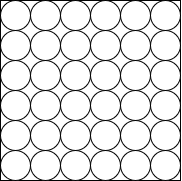
\includegraphics[scale=0.50]{squaretile}
    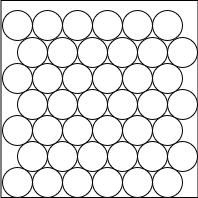
\includegraphics[scale=0.50]{offsetgrid}
    \caption{The left figure is a square grid with each circle has four neighbors, the right is an offset grid where each circle has
    six neighbors. Both diagrams were made using the website Draw.io}
\end{figure}

We can then extend this framework into the third dimension. Given two ways to layer and two directions to layer in, we have four 
possibilities. No matter how we layer, each sphere has at least two neighbors. When we layer using the square method each sphere
gains two neighbors, so if we layer in a grid pattern in both directions we get six total neighbors which means when compressed
it will form a solid with six faces, a cube.

If instead we layer using the offset method each sphere instead gains four neighbors. If we layer one way using the cubic grid,
and the other way using the offset grid we end up with 2 + 2 + 4 or eight faces. Six of the faces lie on a plane and the other
two act as caps, creating hexagonal prisms.  Now this accounts for two of the four possibilities. This is because if we swap
which direction we layer in all it does is rotate the resulting pattern. This means that both patterns result in hexagonal prisms.

When offset layering in two directions things get more complicated. Once we begin stacking 2D layers each sphere will lie between
three spheres on the top and bottom. This means we have 2 base neighbors, then 4 from the 2D packing, and 6 from the 3D packing to
give a total of 12 neighbors, which is a dodecahedron. 

Kepler goes on to claim that the dodecahedron tiling is optimal for stacking spheres, however he does not provide a proof of this 
fact. This portion of the essay is probably the one with the furthest impact on modern mathematics. This assertion is known as 
the Kepler Packing problem and was not proved until at least 1998 \cite{retrospect} with computer assistance. Much like the 
essay that inspired it, the proof was on the boundary of a shift in the philosophy of mathematics. While Kepler was writing in 
the seventeenth century the shift was in the view of mathematics as being the same as the other sciences \cite{snow}, while the change in
the 1990s was about the rise of computers in mathematical proofs.

Kepler accepts this geometric packing as an acceptable explanation for pomegranate seeds forming hexagonal structures, 
however he rejects this for bees. Bee cells are hexagonal prisms, so Kepler begins by looking at unique properties of 
hexagons. Hexagons are one of the few regular polygons which tile the plane with no gaps. The only other polygons with 
this property are triangles and squares, and among these for a given perimeter hexagons have the greatest area \cite[p.19]{kepflake}. 
Kepler does not give formulas for the area to compare, but here are the formulas for their area based on the length of their sides.


\begin{tabular}{c c}
    Triangle & $\frac{\sqrt{3}}{4} a^2$\\
    Square & $a^2$\\ 
    Hexagon & $\frac{3\sqrt{3}}{2} a^2$
\end{tabular}

These formulas come from well known formula for n sided polygons:

\begin{displaymath}
    A = \frac{a^2 n}{4 tan(\frac{\pi}{n})}
\end{displaymath}

If we divide by their perimeter we get:

\begin{tabular}{c c}
    Triangle & $\frac{\sqrt{3}}{12} a$\\
    Square & $\frac{1}{4} a$\\ 
    Hexagon & $\frac{3\sqrt{3}}{12} a$
\end{tabular}

We can see that all formulas are expressible as $\frac{A}{P} = ca$ where the only difference is in a constant coefficient. 
For a square $c=\frac{1}{4}$, for a triangle $c=\frac{\sqrt{3}}{12}$, and for a hexagon $c=\frac{3\sqrt{3}}{12}$. If we 
expand these to decimal we get approximately: 0.25, 0.144, and 0.433 which is the largest constant, implying that for a given 
perimeter hexagons have the largest area.

Unable to continue, Kepler begins to move away from mathematical answers and towards biological and practical answers. 
Perhaps Bees want more area for them to sleep? However a circle would have even more area and although it would leave gaps the 
gaps are not large. Perhaps they have to use a shape which tiles the plane because if they leave gaps the wind might slip through. 
Perhaps God has imprinted the hexagon into bees as some kind of divine knowledge?

But, if hexagons are so divine why do most leaves and plants have five fold symmetry? At this point Kepler acknowledged the limits 
of mathematical thinking. 

At this point I would like to contrast with The Sand Reckoner. Kepler has brought up multiple questions and only answered one. 
Furthermore he completely gives up on several of his questions. When compared to the writing of Archimedes we see less certainty 
and far more willingness to accept ignorance. This can largely be attributed to the purpose and context of these letters, 
Archimedes was writing to a king about his own mathematical achievements \cite{sand}, Kepler was writing to a friend about “Nothing” as he 
would put it \cite[p.3]{kepflake}. However there was also around this time a revisiting of Greek understandings of science and mathematics. According
to the book \textit{Philosophy of mathematics and mathematical practice in the seventeenth century} \cite[p.10-12]{math17}, the seventeenth century saw an 
explosion of new mathematics, and with that renewed debate over what mathematics even is. Is mathematics a science, what kinds 
of mathematical proofs are even valid, what is the role of infinity in mathematics, and so on. Kepler here runs up against the 
boundary of what mathematics can do alone. This work is one in which mathematics takes a center stage but it does not place the 
other sciences below it, which differs from more traditional works which viewed mathematics as something greater and more divine 
than the rest of the sciences.

Kepler proceeds to the namesake of the essay, Why are Snowflakes Hexagonal? He begins with a problem, why are Snowflakes flat? 
After all, when water vapor cools and freezes it seems unlikely only a single flat layer would be cold enough. Also, it was known 
at this time that water vapor expands and changes shape, so it could not be related to the shape of the water before it became vapor. 

At this point Kepler is stuck, so to continue his line of reasoning he makes an assumption. He assumes that when a snowflake forms 
it doesn’t form as a flat hexagonal star, but instead as three rods which intersect. As the snowflake falls the rods collapse into
a flat plane resulting in a hexagon. This is a large assumption and Kepler says he will go as far as he can before checking whether
this is a true assumption. 

In the air we assume that the water vapor is packed in some regular pattern. This can be spread out or compact but it is in some 
regular pattern. If the pattern is in a dodecahedron that doesn’t really help us in our quest to understand freezing, however if 
they are cubic we can immediately see a pattern. If they are in a cubic grid then by freezing from some center point outwards in 
six directions we end up with three rods which we had established could form a hexagonal shape. However we have introduced another 
problem, why would water vapour prefer this pattern? One difference between cubic grids and dodecahedrons is the fact that 
dodecahedron tiling is not as symmetric as a cubic grid to rotations. However beyond just why cubic tiling there are other issues, 
snowflakes are all different sizes and shapes. The only real commonality is that they are all flat when they reach us and have 
six points. 

At this point Kepler can only resort to theology, speculating on the nature and divinity of the octahedron, and cuboid and how 
these might inspire the growth of snowflakes. He moves fully into Platonism and asserts that in the spiritual realm the cube and 
octahedron are the mother and father of the solids. The cube is outwardly focused with six sides and eight vertices. If you take a 
cube and turn it inside out Kepler asserts that you get an octahedron, which is in some sense “inwardly focused”, with eight sides 
and six vertices. One could argue that the snowflakes grew from the three axes of the octahedron because they are “inwardly focused”. 

Another possibility Kepler considers is that the snowflake is related to the shape of man and animals, with a top and bottom, left 
and right, front and back. However he is quick to point out that our bodies have these dimensions for functional reasons, like 
having organs and resilience, reasons that snowflakes need not obey.

However, there is one final problem, Kepler found a snowflake which instead of being a hexagonal start, was a flat solid hexagonal 
plate. This could only mean that our assumption about how snowflakes formed must be incorrect, since rather than three spokes that 
collapse, a plate could only be formed in a single flat piece from the beginning.

At this point Kepler is done and he admits defeat, stating that he has “knocked on the door of chemistry”\cite[p.45]{kepflake}. 

What does The Six Cornered Snowflake mean for historians? It is a window into the idle thoughts and chains of reasoning of a 
scientist like Johannes Kepler. It is also a small window into a shift in the culture of mathematics, a movement from pure reason 
to distinct fields of inquiry and mathematics being somewhat distinct from the sciences. In addition at this time all academic fields 
were permeated with theology and religiosity, a large portion of the debate surrounding the role of mathematics and science is about 
asserting mathematics as divine, and greater than the natural sciences \cite[p.20]{math17} \cite{snow}.

This is also an extremely interesting text since it is about failure. Much of the mathematical literature is about success in some way, and this is a record of one of the many lines of thought that ended inconclusively. It is strange especially compared to something like The Sand Reckoner, which seems to be boastful in its presentation. The problem Kepler tackled here was eventually solved, through a combination of packing, chemistry, and physics we have built a picture of water which forms hexagonal lattices and grows in specific ways depending on temperature. However this essay is less about the triumph of reason and mathematics and more about the ways in which mathematics is limited, and how we came to realize those limitations through failing to answer questions. This story of limitations mirrors the historical events going on around Kepler. The rise of more fields of mathematics lead to re-examination of what mathematics even is, a science, an Aristotelian science, mere intellectual posturing? At the same time in science there was Galileo, Atomic theory, and Kepler’s own contributions which all caused large shifts in scientific thinking and practice.

\printbibliography


\begin{mdframed}
    This Essay did not use Generative AI for any portion of it. All research, diagrams,
    and writing was done by hand without any AI.
\end{mdframed}
\end{document}
